% code_style.tex
\usepackage{xcolor}
\usepackage{tikz}

\newcommand{\greencircle}{%
    
\begin{tikzpicture}
        \fill[green] (0,0) circle (4pt); % Adjust the size here if needed
    \end{tikzpicture}%
}

\newcommand{\greenstar}{%
    
\begin{tikzpicture}[scale=0.22]
        \fill[green] 
            (0,1) 
            -- (0.2245,0.309) 
            -- (1,0.309) 
            -- (0.3633,-0.118) 
            -- (0.5878,-0.809) 
            -- (0,-0.382) 
            -- (-0.5878,-0.809) 
            -- (-0.3633,-0.118) 
            -- (-1,0.309) 
            -- (-0.2245,0.309) 
            -- cycle;
    \end{tikzpicture}%
}

\newcommand{\redcircles}{
    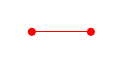
\begin{tikzpicture}[scale=0.75, line cap=round, line join=round]
        % Define coordinates for circles
        \coordinate (A) at (0,0);
        \coordinate (B) at (1,0);
        \coordinate (C) at (2,0);
        \coordinate (D) at (3,0);
        
        % Draw circles
        \foreach \point in {A,B} 
            \fill[red] (\point) circle (2pt);
        
        % Connect circles with lines
        \draw[red] (A) -- (B);
    \end{tikzpicture}%
}

\lstdefinelanguage{Faust}{
    morekeywords={import, process, environment, declare, with, if, else, while, for, int, float, true, false},
    sensitive=true,
    morecomment=[l]{//}, % Line comment
    morecomment=[s]{/*}{*/}, % Block comment
    morestring=[b]", % Strings
}

% Customize the appearance of the code
\lstset{
    language=Faust,
    backgroundcolor=\color{lightgray!20},
    basicstyle=\ttfamily\small,
    keywordstyle=\color{blue}\bfseries,
    stringstyle=\color{orange},
    commentstyle=\color{green}\itshape,
    showstringspaces=false,
    numbers=left,
    numberstyle=\tiny,
    frame=single,
    breaklines=true
}

% Suppress the "Listing #" label and caption text
% \captionsetup[lstlisting]{
%     labelformat=empty,
%     labelsep=none,
%     font=normalfont,
%     skip=0pt
% }
